\documentclass[10pt, hyperref={unicode}]{beamer}

\usepackage[czech]{babel}
\usepackage[utf8]{inputenc}
\usepackage{times}
\usepackage{listings}
\usepackage{graphics}
\usepackage{epigraph}

\setbeamertemplate{footline}[frame number]
%%%%%%%%%%%%%%%%%%%%%%%%%%%%%%%%%%%%%%%%%%%%%%%%%%%%%%%%%%%%%%%%%%%%%%%%%%%%%%%%%%%%%%%%%%%%%%%%%%%
\title{Typografia a~publikovanie\,--\,Projekt~5.}
\author{Binární strom}
\date{\today}

\begin{document}

\maketitle

%%%%%%%%%%%%%%%%%%%%%%%%%%%%%%%%%%%%%%%%%%%%%%%%%%%%%%%%%%%%%%%%%%%%%%%%%%%%%%%%%%%%%%%%%%%%%%%%%%%
\begin{frame}{Motivácia}
	    ``Sometimes it pays to stay in bed on Monday, rather than spending the rest of the week debugging Monday’s code.''
        \\[5pt]
        \rightline{{\rm --- Dan Salomon}}
\end{frame}


\begin{frame}{Obsah}
	\setbeamertemplate{section in toc}[sections numbered]
	\tableofcontents[hideallsubsections]
\end{frame}
%%%%%%%%%%%%%%%%%%%%%%%%%%%%%%%%%%%%%%%%%%%%%%%%%%%%%%%%%%%%%%%%%%%%%%%%%%%%%%%%%%%%%%%%%%%%%%%%%%%

\section{Čo je binárny strom}
\begin{frame}{Binárny strom}
	\begin{itemize}
		\item Binární stromy jsou dynamické datové struktury, ve kterých jsou prvky hierarchicky uspořádány pomocí ukazatelů.
        \bigskip
		\item K~čomu slúžia
			\begin{itemize}
				\item Binární stromy jsou pro informatiku velmi důležité.
				\item Modelují například matematické výrazy.
				\item Modelují binární kódy.
			\end{itemize}
			\bigskip
		\item Při práci se stromem se hojně využívá rekurze.
	\end{itemize}
\end{frame}
%%%%%%%%%%%%%%%%%%%%%%%%%%%%%%%%%%%%%%%%%%%%%%%%%%%%%%%%%%%%%%%%%%%%%%%%%%%%%%%%%%%%%%%%%%%%%%%%%%%

\section{Základné operácie}
\begin{frame}{Základné operácie}
            \begin{itemize}
				\item Počet všech prvků - Ukážka v~sekcii \ref{kod1}
				\item Hledání prvků - Ukážka v~sekcii \ref{kod2}
				\item Přidání nového prvku na určitou pozici ve stromu
				\item Smazání prvku
				\item Vyjmutí celé části stromu – prořezávání (anglicky „pruning“)\\ - 
				Ukážka v~sekcii \ref{kod5}
				\item Přidání celé části do stromu – roubování (anglicky „grafting“)\\ - 
				Ukážka v~sekcii \ref{kod6}
				\item Hledání kořene pro každý uzel
				\item Výška (hloubka) stromu
			\end{itemize}
\end{frame}
%%%%%%%%%%%%%%%%%%%%%%%%%%%%%%%%%%%%%%%%%%%%%%%%%%%%%%%%%%%%%%%%%%%%%%%%%%%%%%%%%%%%%%%%%%%%%%%%%%%

\section{Typy stromov}
\begin{frame}{Typy stromov}
            \begin{itemize}
				\item Strom (graf)
				\begin{itemize}
				    \item  Graf, který je souvislý a neobsahuje žádnou kružnici.
				\end{itemize}
				
				
				\item B-strom
				\begin{itemize}
				    \item  Tato struktura je často používána v~aplikacích, 
				    kdy není celá struktura uložena v~operační paměti (RAM)
				\end{itemize}
			
				
				\item Binární strom (anglicky Binary tree)
				\begin{itemize}
				    \item Datová struktura, používaná k~ukládání a vyhledávání dat v~informatice.
				\end{itemize}
				
				
				\item Halda (datová struktura)
				\begin{itemize}
				    \item   kořenu stromu je vždy prvek s~nejvyšším klíčem (klíč udává funkce x).
				\end{itemize}
			\end{itemize}
\end{frame}
%%%%%%%%%%%%%%%%%%%%%%%%%%%%%%%%%%%%%%%%%%%%%%%%%%%%%%%%%%%%%%%%%%%%%%%%%%%%%%%%%%%%%%%%%%%%%%%%%%%

\label{kod1}
\section{Ukážka kódu}
\begin{frame}{Ukážka kódu počet prvkov}
        \lstinputlisting[language=Octave]{kod1.txt}
\end{frame}
%%%%%%%%%%%%%%%%%%%%%%%%%%%%%%%%%%%%%%%%%%%%%%%%%%%%%%%%%%%%%%%%%%%%%%%%%%%%%%%%%%%%%%%%%%%%%%%%%%%

\label{kod2}

\begin{frame}{Ukážka kódu hľadanie prvkov}
        \lstinputlisting[language=Octave]{kod2.txt}
\end{frame}
%%%%%%%%%%%%%%%%%%%%%%%%%%%%%%%%%%%%%%%%%%%%%%%%%%%%%%%%%%%%%%%%%%%%%%%%%%%%%%%%%%%%%%%%%%%%%%%%%%%

\label{kod5}

\begin{frame}{Ukážka kódu pruning}
        \lstinputlisting[language=Octave]{kod5.txt}
\end{frame}
%%%%%%%%%%%%%%%%%%%%%%%%%%%%%%%%%%%%%%%%%%%%%%%%%%%%%%%%%%%%%%%%%%%%%%%%%%%%%%%%%%%%%%%%%%%%%%%%%%%

\label{kod6}

\begin{frame}{Ukážka kódu grafting}
        \lstinputlisting[language=Octave]{kod6.txt}
\end{frame}
%%%%%%%%%%%%%%%%%%%%%%%%%%%%%%%%%%%%%%%%%%%%%%%%%%%%%%%%%%%%%%%%%%%%%%%%%%%%%%%%%%%%%%%%%%%%%%%%%%%

\section{Ukážka binárneho stromu stromu}
\begin{frame}{Ako vyzerá binárny strom}
        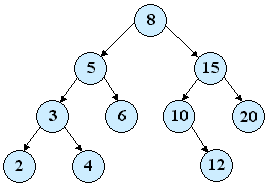
\includegraphics[width=\textwidth]{bvs1.png}
\end{frame}
%%%%%%%%%%%%%%%%%%%%%%%%%%%%%%%%%%%%%%%%%%%%%%%%%%%%%%%%%%%%%%%%%%%%%%%%%%%%%%%%%%%%%%%%%%%%%%%%%%%

\section{Použité zdroje}
\begin{frame}{Použité zdroje}
	\begin{thebibliography}{10}
		\bibitem[Binary tree]{bTree} Binárny strom
		\newblock \texttt{https://bit.ly/3nZV4f4}
		
		\bibitem[Trees]{BskTree} Stromy
		\newblock \texttt{https://bit.ly/3bgv0r7}
		
		\bibitem[Binary tree]{bbTree} Druhy stromov
		\newblock \texttt{https://bit.ly/3uy7IVc}
		
		\bibitem[Binary tree]{kod} Ukážka kódu
		\newblock \texttt{https://bit.ly/3hecZNW}
		
		\bibitem[Binary tree]{kod1} Ukážka kódu
		\newblock \texttt{https://bit.ly/2QZppi2}
		
		\bibitem[Binary tree]{kod2} Ukážka kódu
		\newblock \texttt{https://bit.ly/3vQgcqU}

	\end{thebibliography}
\end{frame}


%%%%%%%%%%%%%%%%%%%%%%%%%%%%%%%%%%%%%%%%%%%%%%%%%%%%%%%%%%%%%%%%%%%%%%%%%%%%%%%%%%%%%%%%%%%%%%%%%%%

\end{document}
